% ****************************************************************************************************
\chapter{Proof of Concept -- Using the Example of SAP HANA Cloud}\label{ch:poc}
% ****************************************************************************************************

\begin{comment}

	GOV 0.6
	TS 0.5
	AS 0.4
	CVP_ITS 0.04
	CVP_ISV 0.05
	CVP_AC 0.01 oder 0.02
	CVP_SI 0.03
	CVP_PC 0.07
	PoAaC_ITS 0.01
	PoAaC_ISV 0.01
	PoAaC_AC 0.02
	PoAaC_SI 0.025
	PoAaC_PC 0.025
	
	Senior Researcher
		expert in 
			a) PaaS development 
			b) Innovation and network theorie

\end{comment}

\begin{figure}[tb]
	\centering
	% ****************************************************************************************************
% Classification Scheme SAP
% ****************************************************************************************************

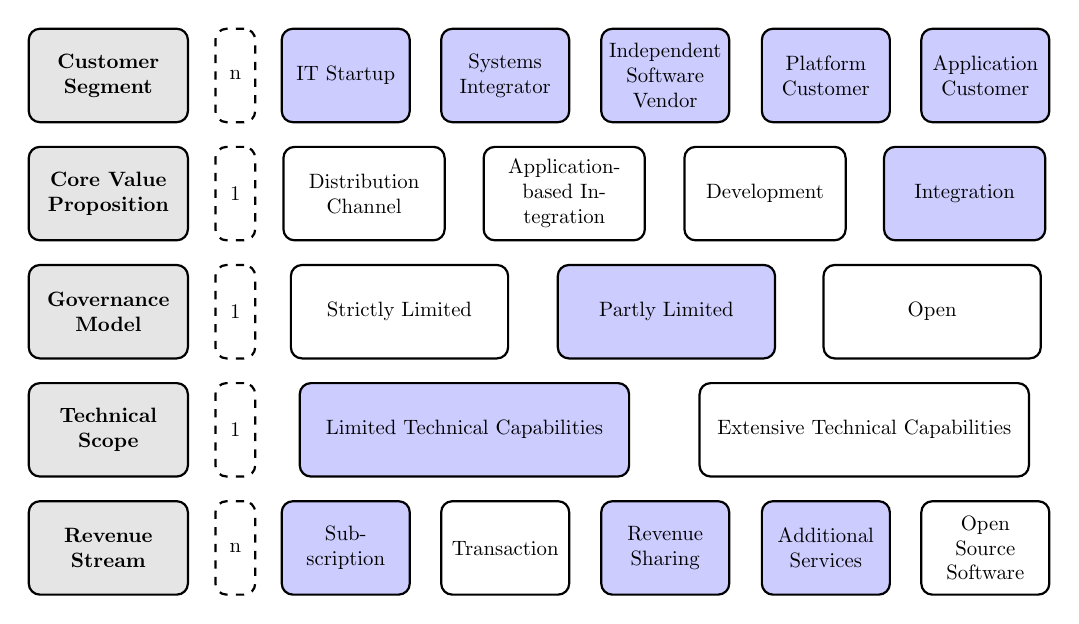
\begin{tikzpicture}[scale=0.75, every node/.style={scale=0.75}]

\node[font={\bfseries},draw,text width=7em,text centered,rectangle,rounded corners,minimum height=4.5em,thick,fill=gray!20] (1) at (-1,8) {Customer Segment};
\node[font={\bfseries},draw,text width=7em,text centered,rectangle,rounded corners,minimum height=4.5em,thick,fill=gray!20] (1) at (-1,6) {Core Value Proposition};
\node[font={\bfseries},draw,text width=7em,text centered,rectangle,rounded corners,minimum height=4.5em,thick,fill=gray!20] (1) at (-1,4) {Governance Model};
\node[font={\bfseries},draw,text width=7em,text centered,rectangle,rounded corners,minimum height=4.5em,thick,fill=gray!20] (1) at (-1,2) {Technical Scope};
\node[font={\bfseries},draw,text width=7em,text centered,rectangle,rounded corners,minimum height=4.5em,thick,fill=gray!20] (1) at (-1,0) {Revenue Stream};

\node[draw,text width=1.25em,text centered,rectangle,rounded corners,minimum height=4.5em,thick,dashed] (1) at (1.15,8) {n};
\node[draw,text width=1.25em,text centered,rectangle,rounded corners,minimum height=4.5em,thick,dashed] (1) at (1.15,6) {1};
\node[draw,text width=1.25em,text centered,rectangle,rounded corners,minimum height=4.5em,thick,dashed] (1) at (1.15,4) {1};
\node[draw,text width=1.25em,text centered,rectangle,rounded corners,minimum height=4.5em,thick,dashed] (1) at (1.15,2) {1};
\node[draw,text width=1.25em,text centered,rectangle,rounded corners,minimum height=4.5em,thick,dashed] (1) at (1.15,0) {n};

\node[draw,text width=5.5em,text centered,rectangle,rounded corners,minimum height=4.5em,thick,fill=blue!20] (1) at (3.02,8) {IT Startup};
\node[draw,text width=5.5em,text centered,rectangle,rounded corners,minimum height=4.5em,thick,fill=blue!20] (1) at (5.72,8) {Systems Integrator};
\node[draw,text width=5.5em,text centered,rectangle,rounded corners,minimum height=4.5em,thick,fill=blue!20] (1) at (8.43,8) {Independent Software Vendor};
\node[draw,text width=5.5em,text centered,rectangle,rounded corners,minimum height=4.5em,thick,fill=blue!20] (1) at (11.15,8) {Platform Customer};
\node[draw,text width=5.5em,text centered,rectangle,rounded corners,minimum height=4.5em,thick,fill=blue!20] (1) at (13.85,8) {Application Customer};

\node[draw,text width=7.1em,text centered,rectangle,rounded corners,minimum height=4.5em,thick] (1) at (3.33,6) {Distribution Channel};
\node[draw,text width=7.1em,text centered,rectangle,rounded corners,minimum height=4.5em,thick] (1) at (6.72,6) {Application-based Integration};
\node[draw,text width=7.1em,text centered,rectangle,rounded corners,minimum height=4.5em,thick] (1) at (10.12,6) {Development};
\node[draw,text width=7.1em,text centered,rectangle,rounded corners,minimum height=4.5em,thick,fill=blue!20] (1) at (13.5,6) {Integration};

\node[draw,text width=9.8em,text centered,rectangle,rounded corners,minimum height=4.5em,thick] (1) at (3.93,4) {Strictly Limited};
\node[draw,text width=9.8em,text centered,rectangle,rounded corners,minimum height=4.5em,thick,fill=blue!20] (1) at (8.45,4) {Partly Limited};
\node[draw,text width=9.8em,text centered,rectangle,rounded corners,minimum height=4.5em,thick] (1) at (12.95,4) {Open};

\node[draw,text width=15.2em,text centered,rectangle,rounded corners,minimum height=4.5em,thick,fill=blue!20] (1) at (5.03,2) {Limited Technical Capabilities};
\node[draw,text width=15.2em,text centered,rectangle,rounded corners,minimum height=4.5em,thick] (1) at (11.8,2) {Extensive Technical Capabilities};

\node[draw,text width=5.5em,text centered,rectangle,rounded corners,minimum height=4.5em,thick,fill=blue!20] (1) at (3.02,0) {Sub-scription};
\node[draw,text width=5.5em,text centered,rectangle,rounded corners,minimum height=4.5em,thick] (1) at (5.72,0) {Transaction};
\node[draw,text width=5.5em,text centered,rectangle,rounded corners,minimum height=4.5em,thick,fill=blue!20] (1) at (8.43,0) {Revenue Sharing};
\node[draw,text width=5.5em,text centered,rectangle,rounded corners,minimum height=4.5em,thick,fill=blue!20] (1) at (11.15,0) {Additional Services};
\node[draw,text width=5.5em,text centered,rectangle,rounded corners,minimum height=4.5em,thick] (1) at (13.85,0) {Open Source Software};

\end{tikzpicture}
	\caption{SAP HANA Cloud Classification}
	\label{fig:cs_sap}
\end{figure}


In conformity with the design cycle of [29], our model has been evaluated against the real world by its reapplication in the context of PaaS business models. In this section, we present a proof of concept study using the 4CaaSt platform . The EU-funded research project 4CaaSt aims to create an advanced PaaS cloud platform which supports the optimized and flexible hosting of Internet-scale multi-tier applications. Hence, the 4CaaSt platform is a development-focused PaaS solution that mainly focuses on the customer segments IT startups, independent software vendors and platform customers. Although 4CaaSt provides an electronic marketplace for cloud-based services, the potential customer segment of application customers is not in direct focus of 4CaaSt, since most services offered on the marketplace consist in software components rather than ready to use applications. This is also indicated in Figure 6, where the main design elements of the 4CaaSt business model are highlighted.

Large parts of the platform are available under open source licenses, hence 4CaaSt pursue an open governance model. 4CaaSt offers extensive technical capabilities by implementing concepts like real application container and bring-your-own-container. As already mentioned, currently large parts of the platform are open source. Nevertheless, a provider of the 4CaaSt platform might charge its customers transaction-based fees.
 
Figure 6. 4CaaSt Business Model Design Elements

In the previous section, six factors influencing the CVP have been discussed. (1) The core value proposition of 4CaaSt which has a direct impact on the CVP is development-focused. This focus seems appropriate for the first three customer segments addressed, but not necessarily for application customers. (2) The open governance model as well as (3) extensive technical capabilities might also positively influence the CVP for IT startups, ISVs and platform customers, although this might not have much influence on application customers. (4) Currently 4CaaSt does not offer any additional services, hence this element will not strengthen the CVP. (5) Platform improvements improve the CVP. However, currently 4CaaSt is free of charge, meaning no revenue is generated that might lead to investments in platform improvements (see self-reinforcing feedback loops R\_2). Nevertheless, improvements of the 4Caast platform might be achieved by developers on an open source basis. However, it could be expected that self-reinforcing feedback loops R\_3 and R\_4 will only be weak. (6) Finally, the market penetration of 4CaaSt is rather low at present. This might change with an increase of the customer base; see self-reinforcing feedback loop (R\_5).
 
Figure 7. 4CaaSt Customer Segment Dynamics

Since 4CaaSt does not address SIs, there are fewer interdependencies between 4CaaSt's customer segments, compare Figure 5 and Figure 7. As a consequence, 4CaaSt will not leverage the two self-reinforcing feedback loops R\_6 and R\_7. Platform modules are developed and provided by ISVs and IT startups and are valuable mainly for platform and application customers. However, 4CaaSt only offers a few ready to use applications that might be used by application customers. Hence, the self-reinforcing feedback loops R\_8, and R\_9 will only have weak effect. Platform customers on the other hand are positively influenced by a high number of available software components and services on which they can build on. Consequently, 4CaaSt will be able to leverage the two self-reinforcing feedback loops R\_10 and R\_11 respectively the cross-sided network effects which are represented by these loops. 

The application of our developed artifacts in the real world scenario of 4CaaSt clearly identifies two emphases, where 4CaaSt might improve their business model. First, 4CaaSt needs to ensure platform improvements. This could on the one hand be accomplished by the platform providers themselves, or 4CaaSt could also create incentives for open source developers. Second, 4CaaSt should definitely improve its value proposition to application customers to utilize critical cross-sided network effects.
